% !TEX program = pdflatex
% TELEMEDICON26 - Team Genesis - CliffForge: six-slide pitch deck (Beamer 16:9, TikZ diagrams).
% Every number below is taken from results/summary.json and results/metrics/*.json (reference run);
% scripts/validate_submission.py checks that this file and README.md agree with those files.
\documentclass[aspectratio=169,10pt]{beamer}

\usepackage[T1]{fontenc}
\usepackage[utf8]{inputenc}
\usepackage[scaled=0.93]{helvet}
\renewcommand{\familydefault}{\sfdefault}
\usepackage{microtype}
\usepackage{amsmath,amssymb}
\usepackage{xcolor}
\usepackage{tikz}
\usetikzlibrary{arrows.meta,calc,positioning,fit,decorations.pathreplacing}
\usepackage[style=authoryear-comp,backend=biber,maxcitenames=2,maxbibnames=3,uniquelist=false,uniquename=false,%
  giveninits=true,useprefix=true,url=false,doi=false,isbn=false,eprint=false]{biblatex}
\addbibresource{references.bib}
\DeclareDelimFormat{nameyeardelim}{\addspace}
\renewcommand*{\finalnamedelim}{\addspace\&\space}
\renewcommand*{\multinamedelim}{\addcomma\space}

% ---------------------------------------------------------------- palette (restrained, flat)
\definecolor{navy}{HTML}{1F2A44}
\definecolor{teal}{HTML}{1B7F8C}
\definecolor{tealmid}{HTML}{7FB8BF}
\definecolor{teallight}{HTML}{E3F1F2}
\definecolor{slate}{HTML}{5B6573}
\definecolor{slatemid}{HTML}{9AA4B2}
\definecolor{slatelight}{HTML}{E9EDF2}
\definecolor{greyline}{HTML}{C5CCD6}
\definecolor{bgc}{HTML}{FBFCFD}
\definecolor{amber}{HTML}{B8741A}

% ---------------------------------------------------------------- beamer look
\usetheme{default}
\usefonttheme{professionalfonts}
\setbeamertemplate{navigation symbols}{}
\setbeamersize{text margin left=8mm,text margin right=8mm}
\setbeamercolor{background canvas}{bg=bgc}
\setbeamercolor{normal text}{fg=navy}
\setbeamercolor{itemize item}{fg=teal}
\setbeamertemplate{itemize item}[square]
\setbeamertemplate{itemize subitem}[square]
\setbeamerfont{itemize/enumerate body}{size=\footnotesize}
\setlength{\leftmargini}{3.2mm}
\setbeamertemplate{frametitle}{%
  \vskip 2.6mm
  {\color{navy}\fontsize{14}{16}\selectfont\bfseries\insertframetitle}\par
  \vskip 1.1mm
  \vskip -3.2mm
  {\color{teal}\rule{10mm}{1.2pt}}\par
  \vskip -1.2mm}
\setbeamertemplate{footline}{%
  \leavevmode\vbox to 7mm{\vss
  \begin{tikzpicture}[remember picture,overlay]
    \draw[greyline,line width=0.4pt] ([xshift=8mm,yshift=5.6mm]current page.south west) -- ([xshift=-8mm,yshift=5.6mm]current page.south east);
    \node[anchor=south west,font=\fontsize{6.5}{7}\selectfont,text=slate] at ([xshift=8mm,yshift=1.6mm]current page.south west)
      {TELEMEDICON26 \quad\textperiodcentered\quad Team Genesis \quad\textperiodcentered\quad CliffForge};
    \node[anchor=south east,font=\fontsize{6.5}{7}\selectfont,text=slate] at ([xshift=-8mm,yshift=1.6mm]current page.south east)
      {\insertframenumber\,/\,\inserttotalframenumber};
  \end{tikzpicture}}}

% ---------------------------------------------------------------- tikz styles
\tikzset{
  >={Stealth[length=2mm]},
  ink/.style={text=navy},
  box/.style={execute at begin node={\hyphenpenalty=10000\exhyphenpenalty=10000\relax},draw=teal,line width=0.8pt,rounded corners=1.2pt,fill=white,align=center,text=navy,
              font=\footnotesize\bfseries,inner sep=3pt,minimum height=9.5mm},
  boxplan/.style={box,draw=slate,dashed,text=slate,fill=slatelight!50},
  lbl/.style={execute at begin node={\hyphenpenalty=10000\exhyphenpenalty=10000\relax},font=\scriptsize,text=slate,align=center,inner sep=1pt},
  arr/.style={->,line width=0.8pt,draw=navy!75},
  arrplan/.style={->,line width=0.8pt,draw=slate,dash pattern=on 2.2pt off 1.8pt},
  panel/.style={draw=greyline,line width=0.5pt,fill=white,inner sep=0pt},
}
% flat aromatic ring: \ring{x}{y}{R}{r}
\newcommand{\ring}[4]{%
  \draw[navy,line width=1pt] ($(#1,#2)+(30:#3)$)--($(#1,#2)+(90:#3)$)--($(#1,#2)+(150:#3)$)--($(#1,#2)+(210:#3)$)--($(#1,#2)+(270:#3)$)--($(#1,#2)+(330:#3)$)--cycle;
  \draw[navy,line width=0.5pt] (#1,#2) circle (#4);}
\newcommand{\sect}[1]{{\color{teal}\bfseries\footnotesize #1}\par\vskip1mm}
\newcommand{\src}[1]{{\color{slate}\fontsize{6.5}{7.5}\selectfont\emergencystretch=4em\tolerance=2000 #1\par}}
\newcommand{\gt}{$\geq$}

\title{CliffForge -- TELEMEDICON26 Pitch Deck}
\author{Team Genesis: Chidwipak Kuppani, Hrishikesh Kurapati}
\subject{Relative-affinity molecular analogue prioritization and activity-cliff analysis}
\keywords{activity cliffs, lead optimization, relative affinity}
\date{}
\begin{document}

% ============================================================== SLIDE 1 - cover
\begin{frame}[plain]
\begin{tikzpicture}[remember picture,overlay]
  \fill[teal] (current page.north west) rectangle ([xshift=3.2mm]current page.south west);
\end{tikzpicture}
\begin{columns}[T,totalwidth=\textwidth]
\column{0.56\textwidth}
\vspace{10mm}
{\color{teal}\bfseries\footnotesize TELEMEDICON26 \quad|\quad PROJECT PITCH DECK}\par\vspace{4mm}
{\color{navy}\fontsize{36}{38}\selectfont\bfseries CliffForge}\par\vspace{3mm}
{\color{slate}\fontsize{12.5}{15}\selectfont Relative-Affinity Molecular Analogue Prioritization and Activity-Cliff Analysis}\par\vspace{4mm}
{\color{slate}\footnotesize Constrained analogue generation \;\textperiodcentered\; relative-affinity scoring \;\textperiodcentered\; uncertainty-aware ranking}\par\vspace{9mm}
{\color{navy}\bfseries Team Genesis}\par\vspace{1.5mm}
{\small Chidwipak Kuppani \;--\; S20230010131 \;--\; UG4\par
 Hrishikesh Kurapati \;--\; S20230010132 \;--\; UG4}\par
\column{0.42\textwidth}
\vspace{4mm}
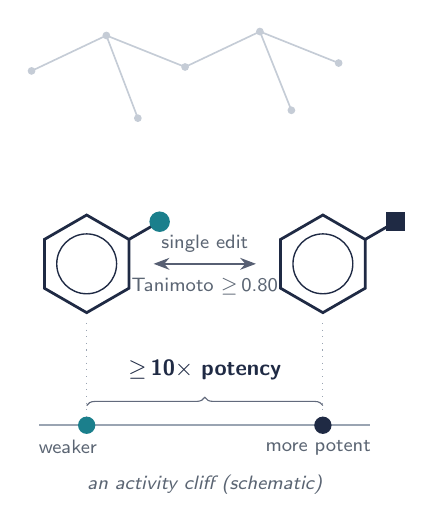
\begin{tikzpicture}[x=1cm,y=1cm]
  % faint molecular-network backdrop
  \coordinate (n1) at (0.0,5.35); \coordinate (n2) at (0.95,5.8); \coordinate (n3) at (1.95,5.4);
  \coordinate (n4) at (2.9,5.85); \coordinate (n5) at (3.9,5.45); \coordinate (n6) at (1.35,4.75); \coordinate (n7) at (3.3,4.85);
  \draw[greyline,line width=0.6pt] (n1)--(n2)--(n3)--(n4)--(n5) (n2)--(n6) (n4)--(n7);
  \foreach \n in {n1,n2,n3,n4,n5,n6,n7} \fill[greyline] (\n) circle (1.4pt);
  % matched pair: ligand A and ligand B differ by one substituent
  \ring{0.7}{2.9}{0.62cm}{0.38cm}
  \draw[navy,line width=1pt] ($(0.7,2.9)+(30:0.62)$) -- ++(30:0.45) coordinate (sa);
  \fill[teal] (sa) circle (0.13);
  \ring{3.7}{2.9}{0.62cm}{0.38cm}
  \draw[navy,line width=1pt] ($(3.7,2.9)+(30:0.62)$) -- ++(30:0.45) coordinate (sb);
  \fill[navy] ($(sb)+(-0.12,-0.12)$) rectangle ($(sb)+(0.12,0.12)$);
  \draw[arr,<->] (1.55,2.9) -- (2.85,2.9);
  \node[lbl,above] at (2.2,3.0) {single edit};
  \node[lbl,below] at (2.2,2.76) {Tanimoto \gt\,0.80};
  % potency track
  \draw[slatemid,line width=0.8pt] (0.1,0.85) -- (4.3,0.85);
  \fill[teal] (0.7,0.85) circle (0.11);
  \fill[navy] (3.7,0.85) circle (0.11);
  \draw[slatemid,dotted] (0.7,2.15) -- (0.7,0.95);
  \draw[slatemid,dotted] (3.7,2.15) -- (3.7,0.95);
  \draw[decorate,decoration={brace,amplitude=3pt},navy!70] (0.7,1.1) -- (3.7,1.1);
  \node[font=\footnotesize\bfseries,text=navy,above] at (2.2,1.3) {\gt\,10$\times$ potency};
  \node[lbl,anchor=north west] at (0.05,0.7) {weaker};
  \node[lbl,anchor=north east] at (4.35,0.7) {more potent};
  \node[font=\scriptsize\itshape,text=slate] at (2.2,0.1) {an activity cliff (schematic)};
\end{tikzpicture}
\end{columns}
\end{frame}

% ============================================================== SLIDE 2 - problem and validation
\begin{frame}{Problem Statement \& Validation}
\begin{columns}[T,totalwidth=\textwidth]
\column{0.465\textwidth}
\sect{What is an activity cliff?}
{\footnotesize Structurally \emph{similar} molecules whose measured potency differs \emph{greatly}: a small edit, a large effect.}\par\vspace{0.5mm}
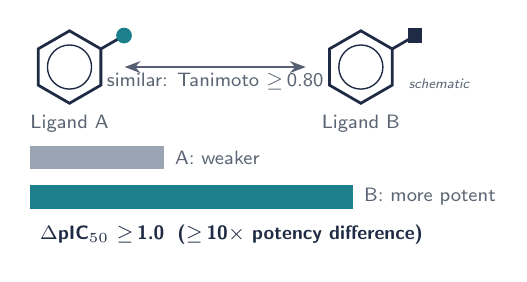
\begin{tikzpicture}[x=1cm,y=1cm]
  \ring{0.7}{1.5}{0.46cm}{0.28cm}
  \draw[navy,line width=1pt] ($(0.7,1.5)+(30:0.46)$) -- ++(30:0.34) coordinate (sa); \fill[teal] (sa) circle (0.1);
  \node[lbl] at (0.7,0.78) {Ligand A};
  \ring{4.4}{1.5}{0.46cm}{0.28cm}
  \draw[navy,line width=1pt] ($(4.4,1.5)+(30:0.46)$) -- ++(30:0.34) coordinate (sb); \fill[navy] ($(sb)+(-0.09,-0.09)$) rectangle ($(sb)+(0.09,0.09)$);
  \node[lbl] at (4.4,0.78) {Ligand B};
  \draw[arr,<->] (1.4,1.5) -- (3.7,1.5);
  \node[lbl,below] at (2.55,1.47) {similar: Tanimoto \gt\,0.80};
  \fill[slatemid] (0.2,0.2) rectangle (1.9,0.5);  \node[lbl,anchor=west] at (2.0,0.35) {A: weaker};
  \fill[teal]    (0.2,-0.3) rectangle (4.3,0.0);  \node[lbl,anchor=west] at (4.4,-0.15) {B: more potent};
  \node[font=\scriptsize\bfseries,text=navy,anchor=north west] at (0.2,-0.38) {$\Delta$pIC$_{50}$ \gt\,1.0 \;(\gt\,10$\times$ potency difference)};
  \node[font=\tiny\itshape,text=slate,anchor=south east] at (5.9,1.1) {schematic};
\end{tikzpicture}\par\vspace{0.5mm}
\begin{itemize}\itemsep0.6mm
  \item \textbf{Why it matters:} chemists must choose which analogues to make; cliffs break ``similar $\Rightarrow$ similar activity''.
  \item Global absolute-activity models and similarity alone can rank close analogues poorly.
\end{itemize}
\column{0.525\textwidth}
\sect{Validation on COVID Moonshot Mpro data}
{\scriptsize 1,102 molecules \;\textperiodcentered\; cliff = Tanimoto \gt\,0.80 \textbf{and} $|\Delta$pIC$_{50}|$ \gt\,1.0}\par\vspace{0.5mm}
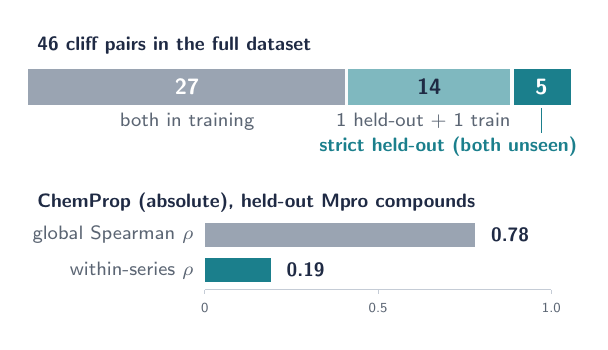
\begin{tikzpicture}[x=1cm,y=1cm]
  \def\u{0.15}
  \node[font=\scriptsize\bfseries,text=navy,anchor=south west] at (0,0.52) {46 cliff pairs in the full dataset};
  \fill[slatemid] (0,0) rectangle (27*\u,0.45);
  \fill[tealmid]  (27*\u,0) rectangle (41*\u,0.45);
  \fill[teal]     (41*\u,0) rectangle (46*\u,0.45);
  \draw[bgc,line width=1.2pt] (27*\u,0) -- (27*\u,0.45) (41*\u,0) -- (41*\u,0.45);
  \node[font=\footnotesize\bfseries,text=white] at (13.5*\u,0.225) {27};
  \node[font=\footnotesize\bfseries,text=navy] at (34*\u,0.225) {14};
  \node[font=\footnotesize\bfseries,text=white] at (43.5*\u,0.225) {5};
  \node[lbl,anchor=north] at (13.5*\u,-0.06) {both in training};
  \node[lbl,anchor=north] at (33.5*\u,-0.06) {1 held-out + 1 train};
  \draw[teal,line width=0.6pt] (43.5*\u,-0.04) -- (43.5*\u,-0.36);
  \node[lbl,anchor=north east,text=teal] at (46*\u+0.12,-0.36) {\textbf{strict held-out (both unseen)}};
  % chart 2 (label column + bars)
  \node[font=\scriptsize\bfseries,text=navy,anchor=north west] at (0,-1.0) {ChemProp (absolute), held-out Mpro compounds};
  \node[lbl,anchor=east] at (2.15,-1.65) {global Spearman $\rho$};
  \fill[slatemid] (2.25,-1.8) rectangle (2.25+0.78*4.4,-1.5);
  \node[font=\scriptsize\bfseries,text=navy,anchor=west] at (2.25+0.78*4.4+0.08,-1.65) {0.78};
  \node[lbl,anchor=east] at (2.15,-2.1) {within-series $\rho$};
  \fill[teal] (2.25,-2.25) rectangle (2.25+0.19*4.4,-1.95);
  \node[font=\scriptsize\bfseries,text=navy,anchor=west] at (2.25+0.19*4.4+0.08,-2.1) {0.19};
  \draw[greyline,line width=0.4pt] (2.25,-2.35) -- (2.25+4.4,-2.35);
  \foreach \t in {0,0.5,1.0} {\draw[greyline] (2.25+\t*4.4,-2.35) -- (2.25+\t*4.4,-2.4); \node[font=\tiny,text=slate,anchor=north] at (2.25+\t*4.4,-2.4) {\t};}
\end{tikzpicture}\par\vspace{-0.5mm}
{\scriptsize Close held-out pairs: 44, containing 5 cliffs (12 test series).}\par
\end{columns}
\vfill
\src{Sources: \parencite{stumpfe2012cliffs,maggiora2006cliffs,vantilburg2023cliffs}; data \parencite{boby2023moonshot}; ChemProp \parencite{yang2019chemprop}; counts: this work.}
\end{frame}

% ============================================================== SLIDE 3 - solution and innovation
\begin{frame}{Proposed Solution \& Innovation}
\begin{columns}[T,totalwidth=\textwidth]
\column{0.5\textwidth}
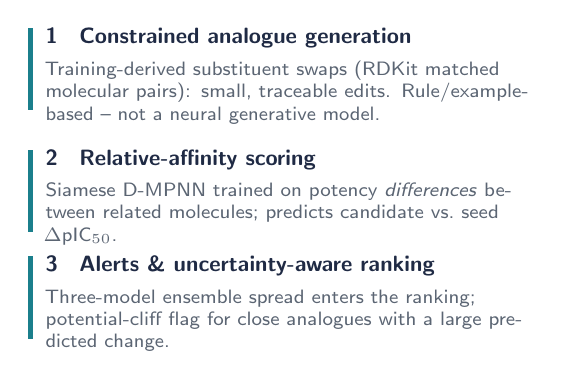
\begin{tikzpicture}[x=1cm,y=1cm]
  \foreach \y/\t/\d in {
    0/{1\;\; Constrained analogue generation}/{Training-derived substituent swaps (RDKit matched molecular pairs): small, traceable edits. Rule/example-based -- not a neural generative model.},
    -1.55/{2\;\; Relative-affinity scoring}/{Siamese D-MPNN trained on potency \emph{differences} between related molecules; predicts candidate vs.\ seed $\Delta$pIC$_{50}$.},
    -2.9/{3\;\; Alerts \& uncertainty-aware ranking}/{Three-model ensemble spread enters the ranking; potential-cliff flag for close analogues with a large predicted change.}} {
    \fill[teal] (0,\y-1.0) rectangle (0.07,\y+0.05);
    \node[anchor=north west,font=\footnotesize\bfseries,text=navy,inner sep=0pt] at (0.22,\y+0.05) {\t};
    \node[anchor=north west,font=\scriptsize,text=slate,text width=6.3cm,align=left,inner sep=0pt] at (0.22,\y-0.37) {\d};
  }
\end{tikzpicture}
\column{0.47\textwidth}
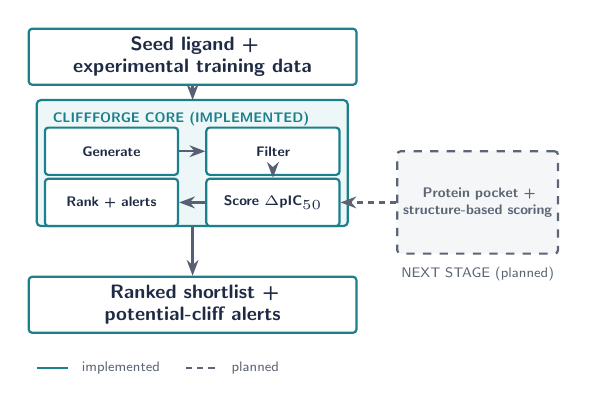
\begin{tikzpicture}[x=1cm,y=1cm]
  \node[box,text width=3.95cm,minimum height=7mm,font=\scriptsize\bfseries] (in) at (1.98,3.7) {Seed ligand +\\experimental training data};
  \draw[teal,line width=0.8pt,rounded corners=1.5pt,fill=teallight!60] (0.0,1.55) rectangle (3.95,3.15);
  \node[font=\tiny\bfseries,text=teal,anchor=north west] at (0.08,3.12) {CLIFFFORGE CORE (IMPLEMENTED)};
  \node[box,text width=1.55cm,minimum height=6mm,font=\tiny\bfseries,inner sep=2pt] (g) at (0.95,2.5) {Generate};
  \node[box,text width=1.55cm,minimum height=6mm,font=\tiny\bfseries,inner sep=2pt] (f) at (3.0,2.5) {Filter};
  \node[box,text width=1.55cm,minimum height=6mm,font=\tiny\bfseries,inner sep=2pt] (r) at (0.95,1.85) {Rank + alerts};
  \node[box,text width=1.55cm,minimum height=6mm,font=\tiny\bfseries,inner sep=2pt] (s) at (3.0,1.85) {Score $\Delta$pIC$_{50}$};
  \draw[arr] (g) -- (f); \draw[arr] (f) -- (s); \draw[arr] (s) -- (r);
  \node[box,text width=3.95cm,minimum height=7mm,font=\scriptsize\bfseries] (out) at (1.98,0.55) {Ranked shortlist + potential-cliff alerts};
  \draw[arr] (in) -- (1.98,3.15); \draw[arr] (1.98,1.55) -- (out);
  % next stage
  \node[boxplan,text width=1.9cm,font=\tiny\bfseries,minimum height=13mm,inner sep=2pt] (fut) at (5.6,1.85) {Protein pocket + structure-based scoring};
  \draw[arrplan] (fut.west) -- (s.east);
  \node[font=\tiny,text=slate,anchor=north] at (5.6,1.15) {NEXT STAGE (planned)};
  % legend
  \draw[teal,line width=0.8pt] (0,-0.25) -- (0.4,-0.25); \node[font=\tiny,text=slate,anchor=west] at (0.45,-0.25) {implemented};
  \draw[slate,dash pattern=on 2.2pt off 1.8pt,line width=0.8pt] (1.9,-0.25) -- (2.3,-0.25); \node[font=\tiny,text=slate,anchor=west] at (2.35,-0.25) {planned};
\end{tikzpicture}
\end{columns}
\par\vspace{0.5mm}
{\scriptsize\color{navy}\textbf{Technology stack:} Python \;\textperiodcentered\; RDKit (transformation transfer, filters) \;\textperiodcentered\; PyTorch Siamese D-MPNN \;\textperiodcentered\; experimental activity data for training \& retrospective evaluation \;\textperiodcentered\; \textcolor{slate}{next: protein-pocket / structure-based scoring}}\par\vspace{0.8mm}
{\scriptsize\color{navy}\textbf{Intended users:} drug-discovery research groups \;\textperiodcentered\; medicinal chemists \;\textperiodcentered\; pharmaceutical and biotechnology lead-optimization teams}\par
\vfill
\src{Sources: matched molecular pairs \parencite{hussain2010mmp,griffen2011mmp}; Siamese networks \parencite{bromley1993siamese}; PyTorch \parencite{paszke2019pytorch}; RDKit (rdkit.org).}
\end{frame}

% ============================================================== SLIDE 4 - technical methodology
\begin{frame}{Technical Methodology}
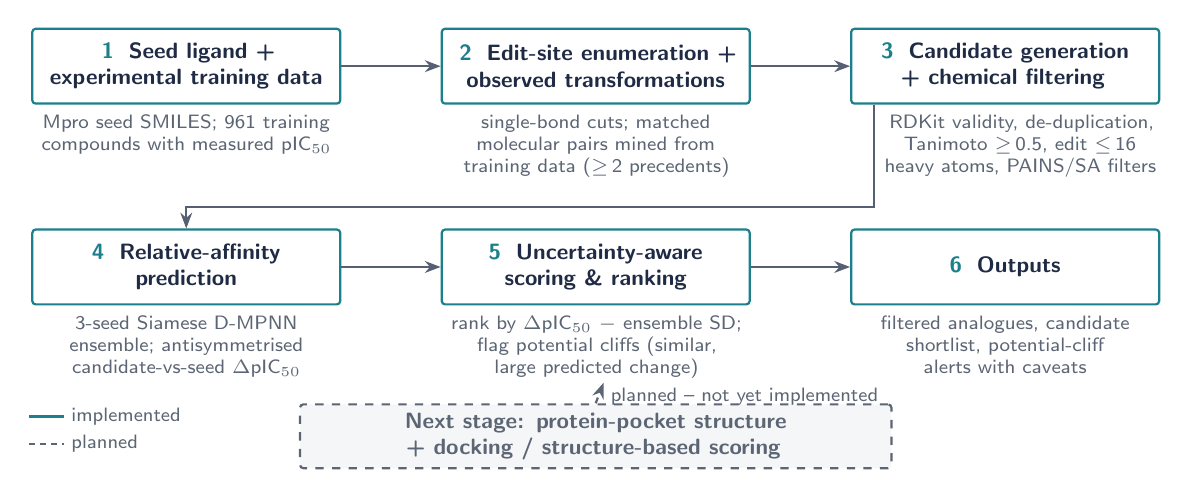
\begin{tikzpicture}[x=1cm,y=1cm]
  \tikzset{st/.style={box,text width=3.7cm,minimum height=9.5mm},
           dl/.style={lbl,text width=3.9cm,anchor=north}}
  % row 1
  \node[st] (n1) at (2.0,0) {\textcolor{teal}{1}\; Seed ligand + experimental training data};
  \node[st] (n2) at (7.2,0) {\textcolor{teal}{2}\; Edit-site enumeration + observed transformations};
  \node[st] (n3) at (12.4,0) {\textcolor{teal}{3}\; Candidate generation + chemical filtering};
  \draw[arr] (n1) -- (n2); \draw[arr] (n2) -- (n3);
  \node[dl] at (2.0,-0.58) {Mpro seed SMILES; 961 training compounds with measured pIC$_{50}$};
  \node[dl] at (7.2,-0.58) {single-bond cuts; matched molecular pairs mined from training data ($\geq$\,2 precedents)};
  \node[dl,text width=3.45cm,anchor=north east] at (14.36,-0.58) {RDKit validity, de-duplication, Tanimoto $\geq$\,0.5, edit $\leq$\,16 heavy atoms, PAINS/SA filters};
  % row 2
  \node[st] (n4) at (2.0,-2.55) {\textcolor{teal}{4}\; Relative-affinity prediction};
  \node[st] (n5) at (7.2,-2.55) {\textcolor{teal}{5}\; Uncertainty-aware scoring \& ranking};
  \node[st] (n6) at (12.4,-2.55) {\textcolor{teal}{6}\; Outputs};
  \draw[arr] (n4) -- (n5); \draw[arr] (n5) -- (n6);
  \draw[arr] ($(n3.south west)+(0.3,0)$) -- ++(0,-1.3) -| (n4.north);
  \node[dl] at (2.0,-3.13) {3-seed Siamese D-MPNN ensemble; antisymmetrised candidate-vs-seed $\Delta$pIC$_{50}$};
  \node[dl] at (7.2,-3.13) {rank by $\Delta$pIC$_{50}$ $-$ ensemble SD; flag potential cliffs (similar, large predicted change)};
  \node[dl] at (12.4,-3.13) {filtered analogues, candidate shortlist, potential-cliff alerts with caveats};
  % future module
  \node[boxplan,text width=7.3cm,minimum height=7.5mm,font=\footnotesize\bfseries] (fut) at (7.2,-4.7) {Next stage: protein-pocket structure + docking / structure-based scoring};
  \draw[arrplan] (fut.north) -- (7.3,-4.02);
  \node[lbl,anchor=west] at (7.35,-4.2) {planned -- not yet implemented};
  \draw[teal,line width=0.8pt] (0.0,-4.45) -- (0.45,-4.45); \node[lbl,anchor=west] at (0.5,-4.45) {implemented};
  \draw[slate,dash pattern=on 2.2pt off 1.8pt,line width=0.8pt] (0.0,-4.8) -- (0.45,-4.8); \node[lbl,anchor=west] at (0.5,-4.8) {planned};
\end{tikzpicture}
\vfill
\src{Sources: matched molecular pairs \parencite{hussain2010mmp}; D-MPNN as in ChemProp \parencite{yang2019chemprop}. Held-out activities are masked at inference.}
\end{frame}

% ============================================================== SLIDE 5 - prototype / proof of concept
\begin{frame}{Prototype / Proof of Concept}
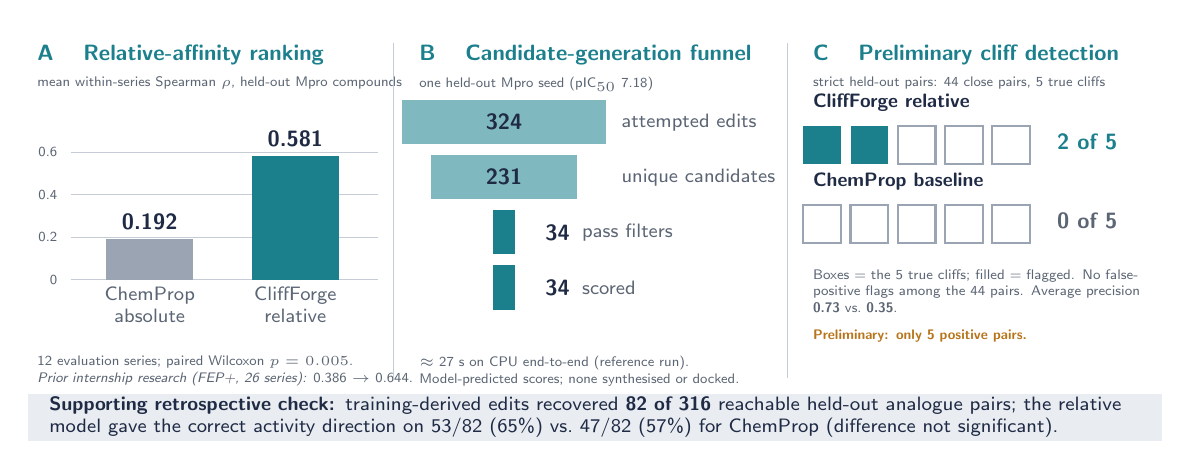
\begin{tikzpicture}[x=1cm,y=1cm]
  \useasboundingbox (0,0.1) rectangle (14.38,-5.2);  % layout box = text width; all content lies inside the page margins
  % ---------------- panel A
  \node[font=\fontsize{7.6}{9}\selectfont\bfseries,text=teal,anchor=north west] at (0,0) {A \;\; Relative-affinity ranking};
  \node[font=\tiny,text=slate,anchor=north west] at (0,-0.4) {mean within-series Spearman $\rho$, held-out Mpro compounds};
  \begin{scope}[shift={(0.55,-3.1)}]
    \draw[greyline,line width=0.4pt] (0,0) -- (3.9,0);
    \foreach \v in {0,0.2,0.4,0.6} {\draw[greyline,line width=0.3pt] (0,\v*2.7) -- (3.9,\v*2.7); \node[font=\tiny,text=slate,anchor=east] at (-0.05,\v*2.7) {\v};}
    \fill[slatemid] (0.45,0) rectangle (1.55,0.192*2.7);
    \fill[teal]     (2.3,0)  rectangle (3.4,0.581*2.7);
    \node[font=\footnotesize\bfseries,text=navy,anchor=south] at (1.0,0.192*2.7) {0.192};
    \node[font=\footnotesize\bfseries,text=navy,anchor=south] at (2.85,0.581*2.7) {0.581};
    \node[lbl,anchor=north] at (1.0,-0.05) {ChemProp\\absolute};
    \node[lbl,anchor=north] at (2.85,-0.05) {CliffForge\\relative};
  \end{scope}
  \node[font=\tiny,text=slate,align=left,anchor=north west] at (0,-3.95) {12 evaluation series; paired Wilcoxon $p=0.005$.\\
    \textit{Prior internship research (FEP+, 26 series):} 0.386 $\to$ 0.644.};
  % ---------------- panel B
  \node[font=\fontsize{7.6}{9}\selectfont\bfseries,text=teal,anchor=north west] at (4.85,0) {B \;\; Candidate-generation funnel};
  \node[font=\tiny,text=slate,anchor=north west] at (4.85,-0.4) {one held-out Mpro seed (pIC$_{50}$ 7.18)};
  \def\fx{6.05}\def\fw{2.6}
  \foreach \y/\n in {-1.1/324, -1.8/231, -2.5/34, -3.2/34} {
    \pgfmathsetmacro{\w}{\fw*\n/324}
    \ifnum \n>100 \def\fc{tealmid} \else \def\fc{teal} \fi
    \fill[\fc] (\fx-\w/2,\y-0.28) rectangle (\fx+\w/2,\y+0.28);
  }
  \node[font=\footnotesize\bfseries,text=navy] at (\fx,-1.1) {324};
  \node[font=\footnotesize\bfseries,text=navy] at (\fx,-1.8) {231};
  \node[font=\footnotesize\bfseries,text=navy,anchor=west] at (\fx+0.4,-2.5) {34};
  \node[font=\footnotesize\bfseries,text=navy,anchor=west] at (\fx+0.4,-3.2) {34};
  \node[lbl,anchor=west,align=left] at (\fx+1.45,-1.1) {attempted edits};
  \node[lbl,anchor=west,align=left] at (\fx+1.45,-1.8) {unique candidates};
  \node[lbl,anchor=west,align=left] at (\fx+0.95,-2.5) {pass filters};
  \node[lbl,anchor=west,align=left] at (\fx+0.95,-3.2) {scored};
  \node[font=\tiny,text=slate,align=left,anchor=north west] at (4.85,-3.95) {$\approx$ 27 s on CPU end-to-end (reference run).\\Model-predicted scores; none synthesised or docked.};
  % ---------------- panel C
  \node[font=\fontsize{7.6}{9}\selectfont\bfseries,text=teal,anchor=north west] at (9.85,0) {C \;\; Preliminary cliff detection};
  \node[font=\tiny,text=slate,anchor=north west] at (9.85,-0.4) {strict held-out pairs: 44 close pairs, 5 true cliffs};
  \foreach \y/\lab/\k/\who in {-1.35/{CliffForge relative}/2/teal, -2.35/{ChemProp baseline}/0/slatemid} {
    \node[font=\scriptsize\bfseries,text=navy,anchor=west] at (9.85,\y+0.5) {\lab};
    \foreach \i in {0,...,4} {
      \ifnum \i<\k \fill[\who] (9.85+\i*0.6,\y-0.28) rectangle (9.85+\i*0.6+0.48,\y+0.2);
      \else \draw[slatemid,line width=0.8pt] (9.85+\i*0.6,\y-0.28) rectangle (9.85+\i*0.6+0.48,\y+0.2); \fi
    }
  }
  \node[font=\footnotesize\bfseries,text=teal,anchor=west] at (12.95,-1.35) {2 of 5};
  \node[font=\footnotesize\bfseries,text=slate,anchor=west] at (12.95,-2.35) {0 of 5};
  \node[font=\tiny,text=slate,anchor=north west,align=left,text width=4.4cm] at (9.85,-2.85) {Boxes = the 5 true cliffs; filled = flagged. No false-positive flags among the 44 pairs. Average precision \textbf{0.73} vs.\ \textbf{0.35}.};
  \node[font=\tiny\bfseries,text=amber,anchor=north west,align=left,text width=4.4cm] at (9.85,-3.62) {Preliminary: only 5 positive pairs.};
  \draw[greyline,line width=0.4pt] (4.65,-0.1) -- (4.65,-4.35) (9.65,-0.1) -- (9.65,-4.35);
  % retrospective strip
  \fill[slatelight] (0,-4.55) rectangle (14.4,-5.15);
  \node[font=\scriptsize,text=navy,anchor=west,text width=13.9cm] at (0.15,-4.85) {\textbf{Supporting retrospective check:} training-derived edits recovered \textbf{82 of 316} reachable held-out analogue pairs; the relative model gave the correct activity direction on 53/82 (65\%) vs.\ 47/82 (57\%) for ChemProp (difference not significant).};
\end{tikzpicture}
\vfill
\src{Sources: ChemProp \parencite{yang2019chemprop}; Moonshot data \parencite{boby2023moonshot}; FEP+ benchmark, prior work \parencite{ross2023fepbenchmark}. All results are new except the FEP+ line. The lead-optimization setting (14 cliffs) gave mixed results and informs the next stage.}
\end{frame}

% ============================================================== SLIDE 6 - impact and next steps
\begin{frame}{Impact, Sustainability \& Next Steps}
\begin{columns}[T,totalwidth=\textwidth]
\column{0.47\textwidth}
\sect{Potential impact (if further validated)}
{\footnotesize More efficient analogue prioritization, with explicit uncertainty, to guide follow-up experiments.}\par\vspace{0.5mm}
\sect{Prospective users (not confirmed partners)}
\begin{itemize}\itemsep0.2mm
  \item Academic drug-discovery groups and medicinal chemistry teams
  \item Biotechnology start-ups and pharmaceutical R\&D
  \item Research collaborations, possibly CRO partners
\end{itemize}\vspace{0.5mm}
\sect{Possible sustainability models (proposals)}
\begin{itemize}\itemsep0.2mm
  \item Open research toolkit
  \item Research collaborations
  \item Optional hosted workflows / institutional integration
\end{itemize}
\column{0.5\textwidth}
\sect{Next-stage roadmap}
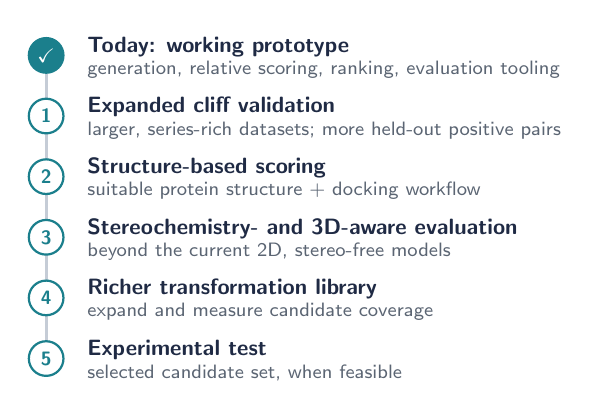
\begin{tikzpicture}[x=1cm,y=1cm]
  \draw[greyline,line width=1pt] (0.22,0.1) -- (0.22,-3.85);
  \foreach \y/\n/\t/\d in {
    -0.05/{\checkmark}/{Today: working prototype}/{generation, relative scoring, ranking, evaluation tooling},
    -0.82/1/{Expanded cliff validation}/{larger, series-rich datasets; more held-out positive pairs},
    -1.59/2/{Structure-based scoring}/{suitable protein structure + docking workflow},
    -2.36/3/{Stereochemistry- and 3D-aware evaluation}/{beyond the current 2D, stereo-free models},
    -3.13/4/{Richer transformation library}/{expand and measure candidate coverage},
    -3.9/5/{Experimental test}/{selected candidate set, when feasible}} {
    \node[draw=teal,fill=white,circle,minimum size=4.4mm,inner sep=0pt,font=\scriptsize\bfseries,text=teal,line width=0.8pt] at (0.22,\y) {\n};
    \node[anchor=west,font=\footnotesize\bfseries,text=navy] at (0.62,\y+0.11) {\t};
    \node[anchor=west,font=\scriptsize,text=slate] at (0.62,\y-0.18) {\d};
  }
  \fill[teal] (0.22,-0.05) circle (0.22); \node[font=\scriptsize\bfseries,text=white] at (0.22,-0.05) {\checkmark};
\end{tikzpicture}
\end{columns}
\vfill
\noindent\colorbox{teallight}{\parbox{\dimexpr\textwidth-2\fboxsep}{\scriptsize\centering\textbf{Value:} relative-affinity learning and activity-cliff-informed analogue prioritization aim to focus effort on the most informative candidates.}}
\vspace{1mm}
\end{frame}

\end{document}
